% =============================================================================================
\chapter{Données et analyse exploratoire}\label{chap:donnees}

% ---------------------------------------------------------------------------------------------
\section{Sources}

Deux sources ouvertes sont utilisées : des prêts réels pour apprendre le risque, et des paramètres sectoriels pour
simuler les indicateurs financiers des projets candidats.

\begin{table}[htbp]
\centering\small
\caption{Sources de données}\label{tab:sources}
\begin{tabularx}{\textwidth}{>{\raggedright\arraybackslash}p{3.2cm}X>{\raggedright\arraybackslash}p{2.4cm}}
\toprule
Source & Contenu et usage & Nature \\
\midrule
SBA 7(a) FOIA~\cite{sba2026} & Prêts garantis par la \textit{Small Business Administration} américaine : montant, part
garantie, durée, taux, secteur NAICS, État, type et âge de l'entreprise, procédure, statut et dates de perte ou de
remboursement. Deux fichiers (exercices 2000-2009 et 2010-2019), instantané au 30 septembre 2026. Sert à apprendre
la probabilité de défaut. & Réelles, domaine public \\
Damodaran~\cite{damodaran2026} & Coût du capital, coût de la dette, bêta, taux d'imposition et part de dette moyens
par secteur d'activité aux États-Unis (janvier 2026). Sert à simuler les flux et à actualiser. & Réelles, publiques \\
Simulation (équipe) & VAN, délai de récupération, DSCR, levier, garanties et score ESG des 40 projets candidats,
générés à partir des paramètres sectoriels (section~\ref{sec:simulation}). & Synthétiques, documentées \\
\bottomrule
\end{tabularx}
\end{table}

Les données SBA sont publiques, volumineuses (plus de 1,2 million de prêts) et indiquent pour chaque prêt s'il a été
remboursé ou perdu : c'est ce qui permet d'apprendre un risque réel. En revanche, aucune base ouverte vérifiée n'associe
l'issue d'un prêt aux comptes financiers du projet financé (VAN, DSCR, TRI). Les consignes autorisant des données
synthétiques à condition d'en décrire la génération, ces indicateurs sont simulés.

% ---------------------------------------------------------------------------------------------
\section{Audit et nettoyage}

Le tableau~\ref{tab:nettoyage} retrace chaque étape, avec le nombre de lignes retirées. Les statuts ont été comptés
avant de construire la cible : le fichier en contient cinq (\code{P I F} pour remboursé, \code{CHGOFF} pour perdu,
\code{CANCLD} pour annulé, \code{EXEMPT} et \code{COMMIT}), et non treize comme certaines documentations le laissaient
penser. L'écriture \code{P I F} est la seule variante présente.

\begin{table}[htbp]
\centering
\small\setlength{\tabcolsep}{4pt}
\caption{Audit et nettoyage des données SBA}\label{tab:nettoyage}
\begin{tabular}{lr}
\toprule
Étape & Lignes \\
\midrule
Lignes brutes (deux fichiers FY2000-2009 et FY2010-2019) & 1\,236\,084 \\
Lignes à colonnes décalées (statut invalide) & -47 \\
Doublons exacts & -1\,414 \\
Sans date de premier versement (dont 147\,990 annulés) & -149\,575 \\
Statut EXEMPT (issue inconnue) & -49\,929 \\
Versés depuis moins de 60 mois & -122 \\
Identifiants hachés en double & -2\,426 \\
Approuvés hors 2000-2016 & -122\,538 \\
\textbf{Prêts conservés} & \textbf{910\,033} \\
\bottomrule
\end{tabular}
\end{table}


Trois décisions méritent une justification :
\begin{itemize}
  \item \textbf{Les prêts sans date de premier versement sont écartés} : sans cette date, on ne peut pas savoir si la
        perte survient dans les 60 mois. Il s'agit presque exclusivement de prêts annulés (147\,990 sur 149\,575).
  \item \textbf{Les prêts au statut EXEMPT sont écartés} : leur issue est inconnue.
  \item \textbf{Seuls les prêts versés depuis au moins 60 mois sont gardés} : un prêt récent sans défaut n'est pas
        un prêt sain, simplement un prêt dont l'issue n'est pas encore connue.
\end{itemize}
Les colonnes connues seulement après l'octroi (statut, dates de remboursement et de perte, montant perdu, vente sur
le marché secondaire) et les données personnelles (nom, adresse, banque) sont supprimées dès cette étape. Chaque prêt
reçoit un identifiant haché, ce qui garantit qu'aucun nom d'emprunteur ne circule dans la suite du pipeline.

\section{Construction de la cible et séparation temporelle}

Un prêt vaut $y = 1$ s'il est au statut \code{CHGOFF} et que sa date de perte survient au plus 60 mois après le premier
versement. Les 66\,652 prêts perdus plus tard comptent comme $y = 0$ : une perte très tardive ne dépend plus de l'état
du dossier à l'octroi. Les prêts sont ensuite séparés selon leur exercice d'approbation
(tableau~\ref{tab:blocs}), avant tout calcul qui apprend des données.

\begin{table}[htbp]
\centering
\small\setlength{\tabcolsep}{4pt}
\caption{Séparation temporelle des prêts SBA 7(a)}\label{tab:blocs}
\begin{tabular}{llrrrl}
\toprule
Bloc & Années & Prêts & Défauts & Taux & Rôle \\
\midrule
Entraînement & 2000-2012 & 723\,663 & 97\,535 & 13,48\,\% & apprentissage \\
Validation & 2013-2014 & 82\,384 & 2\,939 & 3,57\,\% & réglage, calibration, choix \\
Test & 2015-2016 & 103\,986 & 4\,415 & 4,25\,\% & mesure finale (lue une fois) \\
\bottomrule
\end{tabular}
\end{table}


% ---------------------------------------------------------------------------------------------
\section{Analyse exploratoire}

\subsection{Un changement de régime marqué}

La figure~\ref{fig:annee} montre l'évolution du taux de défaut par année d'approbation. Il passe d'environ 6,5\,\% en
2000 à 28\,\% pour les prêts accordés en 2007, juste avant la crise financière, puis retombe sous 5\,\% à partir de
2011. Le bloc d'entraînement contient donc la crise, contrairement aux blocs de validation et de test : son taux de
défaut (13,5\,\%) est environ trois fois plus élevé. Cette observation a deux conséquences méthodologiques : les
probabilités brutes d'un modèle appris sur 2000-2012 seront trop élevées pour 2015-2016, d'où la calibration sur la
validation ; et toute grandeur calculée sur l'entraînement (comme un taux de défaut de référence) doit être utilisée
avec précaution.

\begin{figure}[htbp]
  \centering
  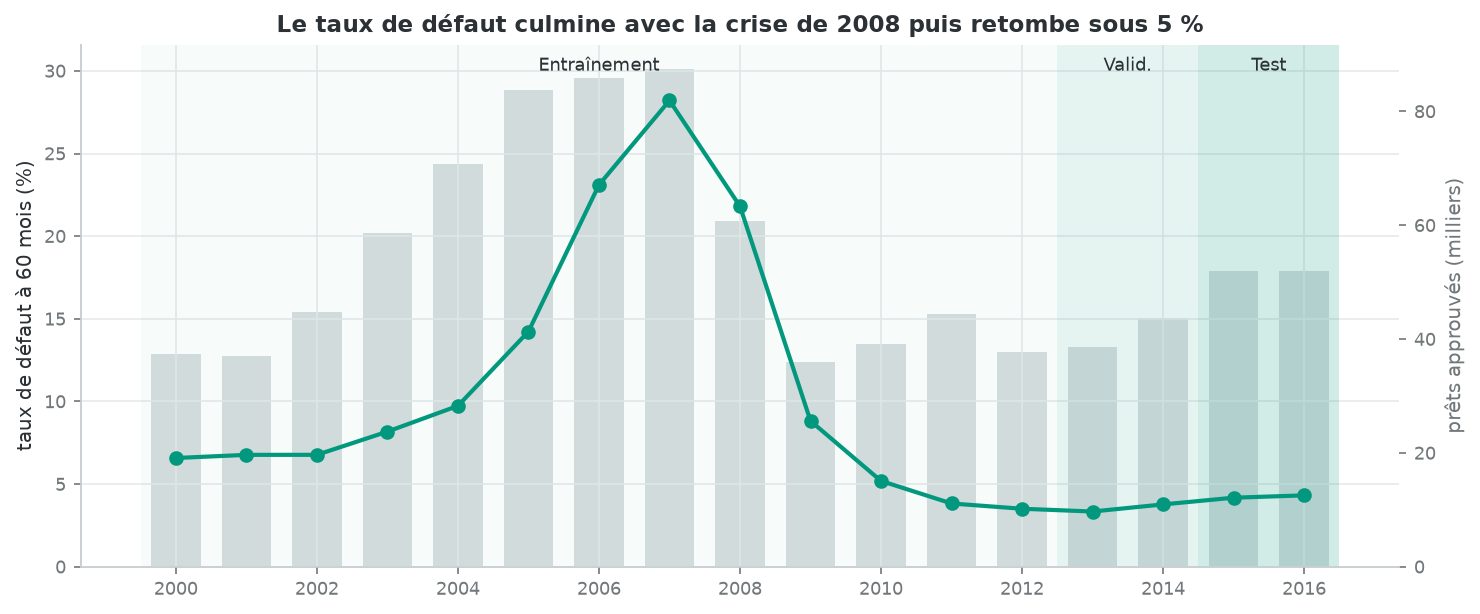
\includegraphics[width=\textwidth]{fig_defaut_par_annee.png}
  \caption{Taux de défaut à 60 mois (courbe) et nombre de prêts approuvés (barres) par année. Les zones colorées
  indiquent les blocs d'entraînement, de validation et de test.}
  \label{fig:annee}
\end{figure}

\subsection{Des classes déséquilibrées}

Le défaut est minoritaire dans les trois blocs (figure~\ref{fig:desequilibre}), de 3,6 à 13,5\,\% des prêts. Ce
déséquilibre justifie le choix de l'AUPRC et du score de Brier, en plus de l'AUROC, et un seuil de décision choisi sur
la validation plutôt que le seuil naïf de 0,5.

\begin{figure}[htbp]
  \centering
  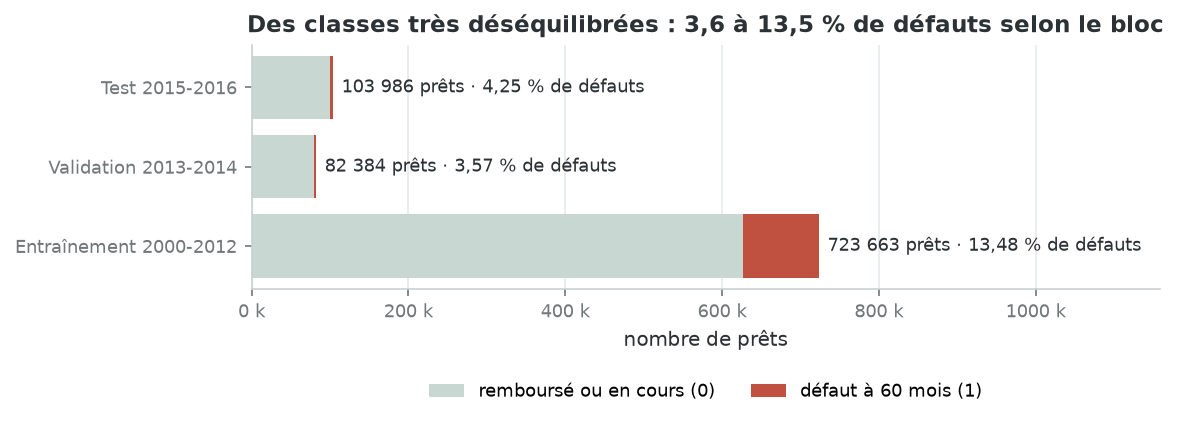
\includegraphics[width=0.85\textwidth]{fig_desequilibre.png}
  \caption{Répartition des prêts par issue dans chaque bloc.}
  \label{fig:desequilibre}
\end{figure}

\subsection{Secteur, montant et caractéristiques du prêt}

Le risque varie fortement selon le secteur (figure~\ref{fig:secteur}) : de 5,2\,\% dans l'agriculture à 19,0\,\% dans
l'immobilier, sur la période d'entraînement. Il décroît avec le montant (figure~\ref{fig:montant}) : les 10\,\% de
prêts les plus petits font défaut près de six fois plus souvent que les 10\,\% les plus gros (19,9\,\% contre
3,5\,\%). Les petits prêts, souvent accordés par des procédures simplifiées, sont octroyés à des entreprises plus
fragiles.

\begin{figure}[htbp]
  \centering
  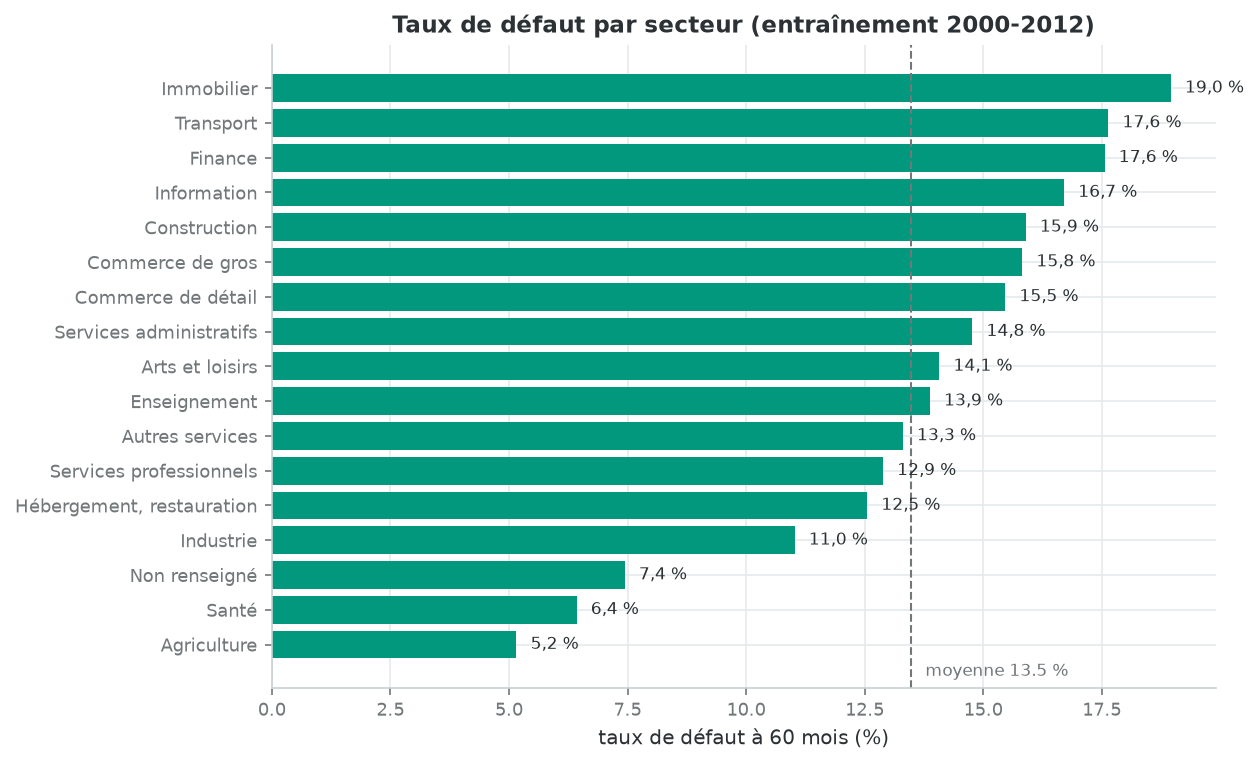
\includegraphics[width=0.8\textwidth]{fig_defaut_par_secteur.png}
  \caption{Taux de défaut par secteur d'activité (secteurs d'au moins 2\,000 prêts, entraînement). La ligne
  pointillée indique la moyenne.}
  \label{fig:secteur}
\end{figure}

\begin{figure}[htbp]
  \centering
  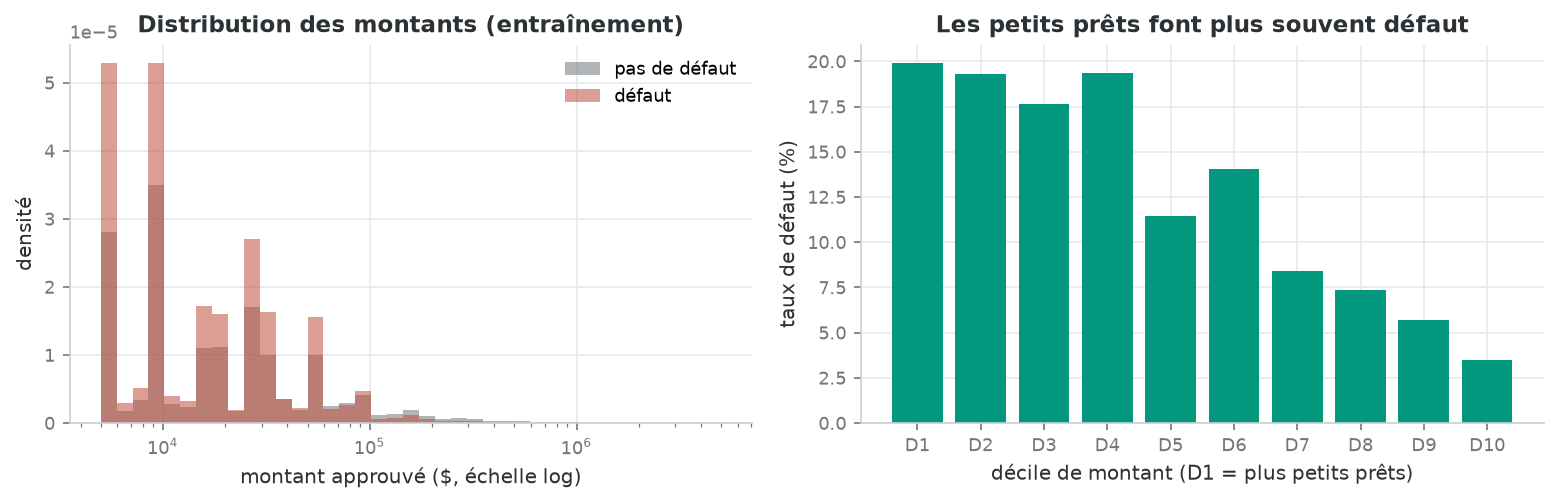
\includegraphics[width=\textwidth]{fig_montant.png}
  \caption{Distribution des montants selon l'issue (gauche) et taux de défaut par décile de montant (droite).
  Les pics de la distribution correspondent aux montants ronds (10\,000, 25\,000, 50\,000\,\$\dots).}
  \label{fig:montant}
\end{figure}

La figure~\ref{fig:categorielles} montre l'effet de quatre caractéristiques. La procédure d'octroi est la plus
discriminante : les programmes express (\textit{Community Express}, \textit{SBA Express}) ont des taux de défaut
deux à six fois plus élevés que les prêts instruits par des prêteurs certifiés. Les lignes de crédit renouvelables
sont plus risquées que les prêts amortissables. L'absence de taux d'intérêt renseigné est associée à un risque élevé,
mais c'est un artefact temporel : le taux n'est pas renseigné pour 79\,\% des prêts d'entraînement, surtout anciens
(figure~\ref{fig:manquants}), et il l'est pour tous les prêts de validation et de test.

\begin{figure}[htbp]
  \centering
  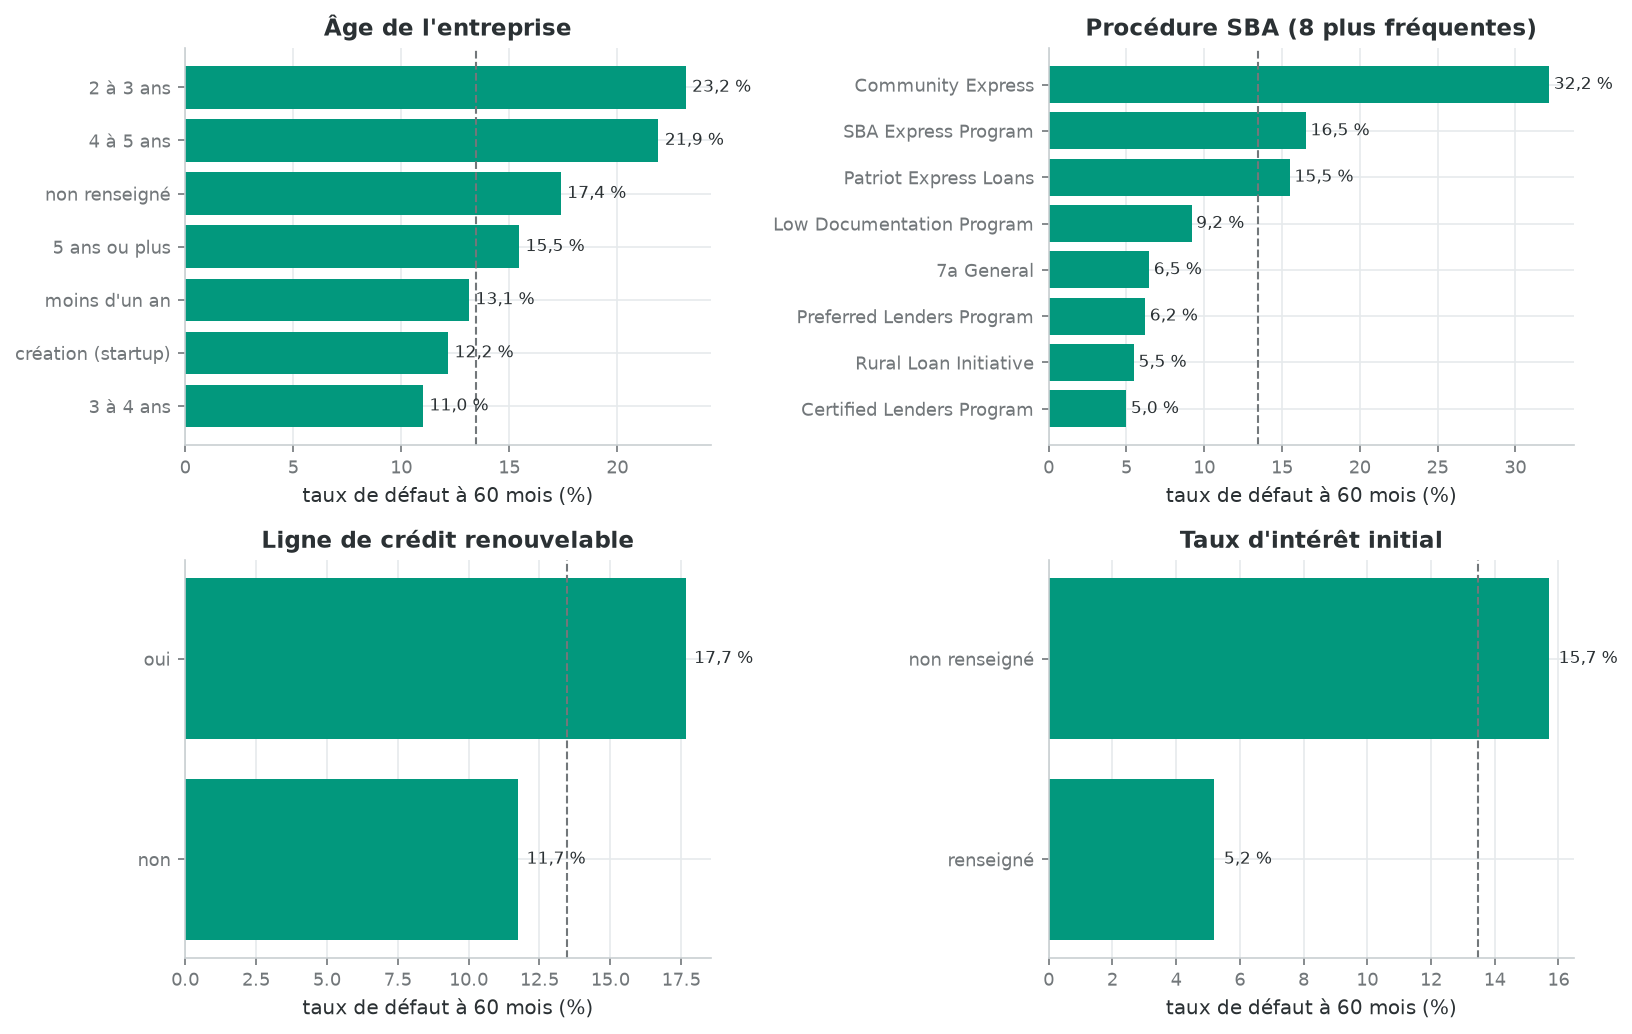
\includegraphics[width=\textwidth]{fig_variables_categorielles.png}
  \caption{Taux de défaut selon l'âge de l'entreprise, la procédure SBA, la ligne renouvelable et la présence du
  taux d'intérêt (entraînement ; ligne pointillée : moyenne).}
  \label{fig:categorielles}
\end{figure}

\begin{figure}[htbp]
  \centering
  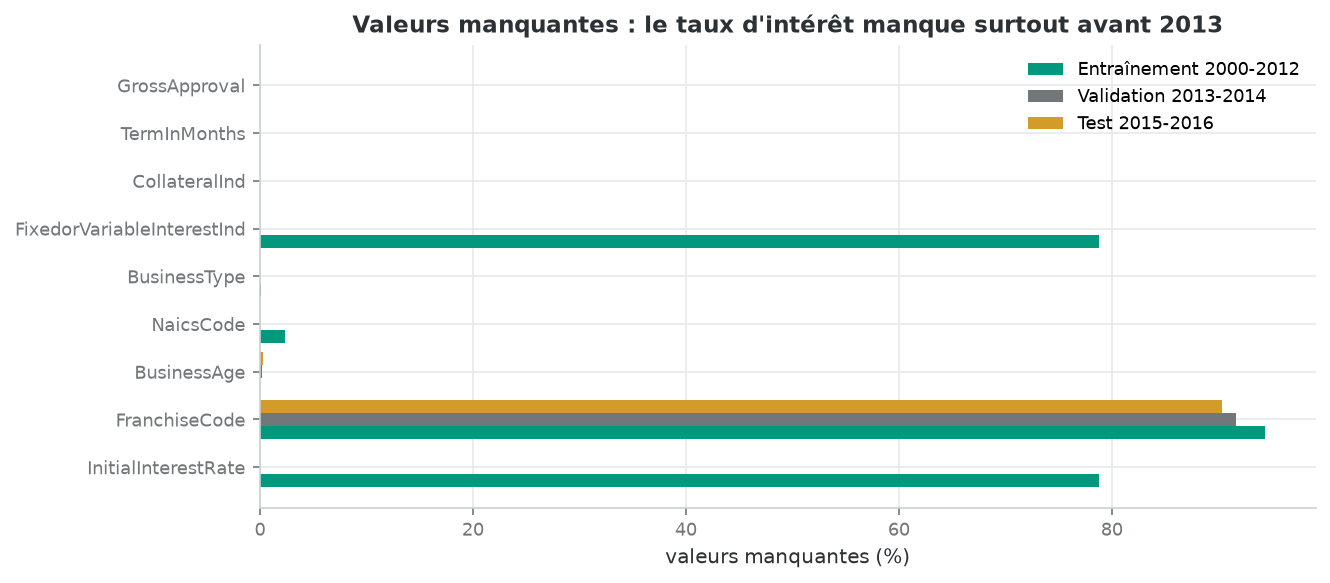
\includegraphics[width=0.85\textwidth]{fig_valeurs_manquantes.png}
  \caption{Part de valeurs manquantes par variable et par bloc. L'absence de code de franchise signifie
  \og pas de franchise \fg{} et n'est pas une donnée manquante.}
  \label{fig:manquants}
\end{figure}

\subsection{Une fuite de données détectée}\label{sec:fuite}

La durée du prêt est la variable la plus liée au défaut (figure~\ref{fig:duree}, gauche) : 28\,\% de défauts pour les
prêts de 60 mois ou moins, contre 2\,\% au-delà de 120 mois. Un premier modèle utilisant la durée exacte
(\code{TermInMonths}) atteignait une AUROC de 0,96 sur la validation, valeur trop élevée pour être crédible en
scoring de PME. L'examen de la variable a révélé la cause : les durées \og rondes \fg{} (12, 24, 60, 84, 120 mois)
correspondent à 1,6\,\% de défauts, les durées \og non rondes \fg{} (87, 129 mois\dots) à 34,9\,\%
(figure~\ref{fig:duree}, droite). La durée enregistrée est modifiée \emph{après} l'octroi lorsque le prêt tourne mal
(restructuration, résiliation) : elle contient en partie l'issue.

\begin{figure}[htbp]
  \centering
  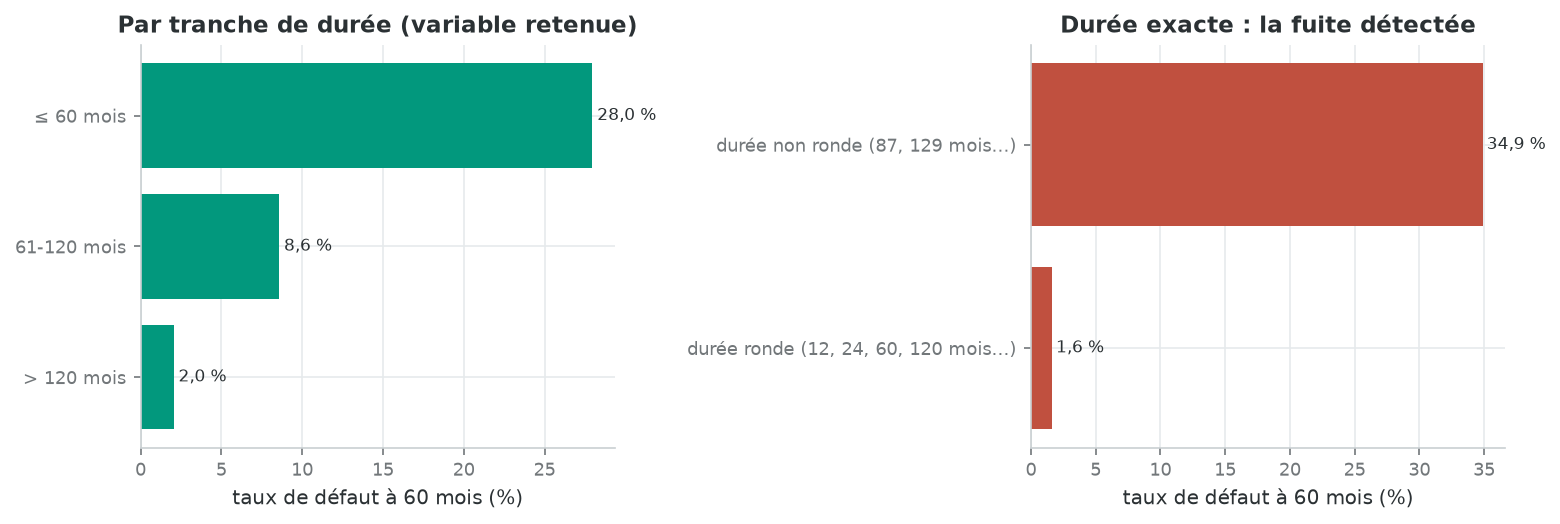
\includegraphics[width=\textwidth]{fig_duree.png}
  \caption{Taux de défaut par tranche de durée (gauche, variable retenue) et selon que la durée exacte est ronde ou
  non (droite) : la durée exacte révèle l'issue du prêt.}
  \label{fig:duree}
\end{figure}

\begin{encadre}[Correction retenue]
La durée exacte est remplacée par trois tranches larges : 60 mois ou moins, 61 à 120 mois, plus de 120 mois. Des tests
rapides donnaient une AUROC de validation de 0,96 avec la durée exacte, 0,81 avec cinq tranches, 0,79 avec trois
tranches et 0,67 sans aucune information de durée. Trois tranches conservent l'essentiel de l'information
légitime (un prêt court finance souvent un besoin plus risqué) sans laisser passer la fuite. C'est un écart assumé
par rapport à la liste de variables prévue initialement. La même vérification sur le taux d'intérêt n'a révélé
aucune anomalie.
\end{encadre}

% ---------------------------------------------------------------------------------------------
\section{Variables du modèle et prétraitement}

Les trois modèles utilisent exactement les mêmes 13 variables, toutes connues au moment de la demande
(tableau~\ref{tab:variables}).

\begin{table}[htbp]
\centering\small
\caption{Variables du modèle de risque}\label{tab:variables}
\begin{tabularx}{\textwidth}{>{\raggedright\arraybackslash}p{4cm}X}
\toprule
Variable & Construction \\
\midrule
Montant (log) & $\log(1 + \text{montant approuvé})$ \\
Part garantie & montant garanti par la SBA / montant approuvé \\
Taux d'intérêt initial & tel quel, avec une indicatrice \og taux non renseigné \fg{} \\
Tranche de durée & 3 tranches (section~\ref{sec:fuite}) \\
Taux fixe ou variable, ligne renouvelable & catégorielles \\
Secteur & deux premiers chiffres du code NAICS \\
État, type d'entreprise, âge de l'entreprise & catégorielles \\
Franchise & oui si un code de franchise est renseigné \\
Procédure SBA & catégorielle (express, prêteurs certifiés, etc.) \\
\bottomrule
\end{tabularx}
\end{table}

Deux variables disponibles sont volontairement exclues pour éviter un \emph{double comptage}. Le nombre d'emplois
soutenus devient le critère multicritère \og emplois par million \fg{}, et l'indicateur de garantie réelle sert au
critère \og couverture par les garanties \fg{}. Les garder dans le modèle ferait compter deux fois le même fait, une
fois dans la probabilité de défaut et une fois dans le critère.

Pour la régression logistique, les variables numériques sont imputées par la médiane puis standardisées, et les
catégorielles codées en indicatrices (les modalités rares, moins de 200 prêts, sont regroupées). Ces
transformations sont des \textit{pipelines} scikit-learn ajustés sur l'entraînement uniquement. L'EBM et LightGBM
traitent les variables catégorielles et les valeurs manquantes nativement ; pour LightGBM, les modalités sont
apprises sur l'entraînement et une modalité inconnue devient une valeur manquante.
